\documentclass[11pt,a4paper,twocolumn]{article}

% === Core Packages ===
\usepackage[margin=2cm]{geometry}
\usepackage[utf8]{inputenc}
\usepackage[T1]{fontenc}
\usepackage{times}
\usepackage{amsmath,amssymb}
\usepackage{graphicx}
\usepackage{booktabs}
\usepackage{float}
\usepackage{enumitem}
\usepackage{tikz}
\usepackage{pgfplots}
\pgfplotsset{compat=1.18}
\usetikzlibrary{arrows.meta,shapes.geometric,positioning,calc,decorations.markings,fit,backgrounds}

% === Citation (IEEE style) ===
\usepackage[numbers,sort&compress]{natbib}
\bibliographystyle{IEEEtranN}

% === Hyperref ===
\usepackage[hidelinks]{hyperref}
\usepackage{xurl}

% === Settings ===
\setlength{\parindent}{1em}
\setlength{\parskip}{0.3em}

% === PDF metadata ===
\hypersetup{
  pdftitle={Rede de Reputação Descentralizada: Um Arcabouço para a Organização Natural da Sociedade},
  pdfauthor={Pavel Kudrna},
  pdfsubject={Personix — a decentralized reputation network},
  pdfkeywords={Personix, decentralized reputation, reputation social network,
    decentralized identifiers, DID, meritocracy, censorship resistance},
}

% === Title ===
\title{\textbf{Rede de Reputação Descentralizada:\\Um Arcabouço para a Organização Natural da Sociedade}}
\author{Pavel Kudrna\\Personix Project --- \url{https://personix.org}\\Prague, Czechia\\Draft v1 --- March 2026}
\date{}

\begin{document}
\maketitle

% ============================================================
% ABSTRACT
% ============================================================
\begin{abstract}
O senso de justiça---a convicção de que os males são reparados e o mérito é recompensado---é a mais forte força de coesão da sociedade. Quando as instituições centralizadas de governança não conseguem oferecer esse senso porque o custo de fazer valer um direito excede o próprio valor do direito, a coesão social se corrói. As estruturas institucionais atuais não conseguem resolver uma classe significativa de disputas sistematicamente pela mesma razão pela qual o planejamento central falha em alocar recursos: por meio da assimetria de informação, de ciclos de retroalimentação ausentes e da desconexão entre os tomadores de decisão e as consequências de suas decisões. Este artigo apresenta uma Rede Social de Reputação (RSN): uma camada de comunicação descentralizada, incorruptível e resistente à censura, construída sobre Identificadores Descentralizados (DIDs), que permite a participantes pseudônimos publicar, verificar e consumir informações de reputação sobre comportamentos do mundo real. O mecanismo central repousa sobre três princípios de projeto: (1)~uma estrutura de custo assimétrica em que ler dados de reputação é barato, mas escrever exige esforço verificável; (2)~um protocolo não determinístico de seleção de verificadores baseado em hashing consistente, que precifica alegações radicais por meio de custos de iteração crescentes; e (3)~um modelo de autoridade de reputação orientado pelo mercado, no qual verificadores privados apostam sua reputação acumulada na exatidão das alegações que endossam. A arquitetura resultante produz meritocracia emergente sem coordenação central e viabiliza um caminho de migração gradual e reversível a partir dos sistemas atuais administrados pelo Estado.
\end{abstract}

% ============================================================
% 1. INTRODUCTION
% ============================================================
\section{Introdução}

\subsection{O Problema da Confiança Centralizada}

A governança moderna repousa sobre um pressuposto fundamental: o de que instituições centralizadas podem mediar a confiança entre estranhos em larga escala. Tribunais julgam disputas. Cartórios certificam a propriedade. Órgãos reguladores fazem cumprir padrões. Essas instituições foram concebidas numa era em que a informação era escassa, a comunicação era lenta e a delegação de autoridade a um órgão central era o único mecanismo de coordenação viável. A governança centralizada, no entanto, falha pelas mesmas razões estruturais que o planejamento central: assimetria de informação, ciclos de retroalimentação ausentes e desconexão entre os tomadores de decisão e as consequências de suas decisões.

O pressuposto falha, por exemplo, quando o custo da mediação institucional excede o valor da disputa. Considere um inquilino que descobre que o apartamento alugado carece de um certificado de segurança elétrica legalmente exigido---uma condição que representa perigo imediato à vida. O direito legal do inquilino de rescindir o contrato é inequívoco. Ainda assim, o custo de fazer valer esse direito pelo sistema judiciário excede o valor monetário do depósito e dos danos devidos, mesmo incluindo a eventual indenização prevista em lei~\cite{czcourtfees}. A resposta racional é absorver a perda e sair.

Isso não é um caso patológico e excepcional. É a experiência padrão para uma classe significativa de disputas em que o dano é real, mas o valor monetário em jogo fica abaixo do limiar a partir do qual a execução institucional se torna economicamente racional. O resultado é um sistema que favorece estruturalmente os maus atores: aqueles que prejudicam outros em volumes abaixo desse limiar podem agir com impunidade, porque o custo de buscar justiça recai sobre a parte lesada.

O exemplo acima é extraído do ambiente jurídico do autor---o sistema de direito civil tcheco. Em outras tradições jurídicas---o direito consuetudinário baseado em precedentes (common law), o direito costumeiro, os sistemas mistos---a justiça falha de maneiras diferentes e em graus diferentes, dependendo das especificidades culturais e processuais da jurisdição. É provável que os leitores reconheçam exemplos equivalentes em seu próprio contexto. O que é estruturalmente universal é o padrão: disputas cujo valor fica abaixo do limiar de execução economicamente racional terminam com a perda sendo absorvida pela parte lesada. A RSN não promete justiça perfeita---ela apenas reduz a vantagem estrutural de que os maus atores desfrutam quando a execução institucional é antieconômica.

\subsection{Por que as Soluções Existentes Ficam Aquém}

\textbf{Arcabouços de Identidade Descentralizada (DID)}~\cite{did2022} fornecem mecanismos criptográficos para a gestão de identidade autossoberana, mas concentram-se sobretudo na verificação de identidade sem abordar a questão mais ampla da reputação comportamental.

\textbf{Tokens Soulbound (SBTs)}~\cite{weyl2022} captam a percepção de que a reputação é intransferível, mas dependem de uma infraestrutura de blockchain com restrições de escalabilidade e não tratam dos incentivos econômicos que governam a inserção de informação. Conceitos correlatos, como tokens de mérito (por exemplo, Liberland), compartilham uma filosofia semelhante, mas permanecem atrelados a arcabouços jurisdicionais específicos.

\textbf{Organizações Autônomas Descentralizadas (DAOs)}~\cite{buterin2014} implementam governança por meio de contratos inteligentes, mas reproduzem dinâmicas plutocráticas em que a influência é proporcional ao capital. O voto quadrático~\cite{buterin2019} mitiga isso parcialmente, mas limita a adoção prática. As DAOs também enfrentam o \emph{problema do oráculo} fundamental: contratos inteligentes não conseguem verificar de forma confiável estados do mundo real sem uma fonte externa confiável, e esse problema não tem solução geral dentro da arquitetura de blockchain.

Nenhum sistema existente combina descentralização, resistência à censura, pseudonimato, custo de entrada verificável e consenso emergente.

\subsection{Contribuições}

Este artigo apresenta as seguintes contribuições:
\begin{enumerate}[nosep]
\item Definição da \textbf{Rede Social de Reputação (RSN)}, um protocolo descentralizado que estende o arcabouço DID para suportar a troca bilateral de reputação.
\item Um \textbf{protocolo não determinístico de seleção de verificadores} baseado em hashing consistente~\cite{karger1997}.
\item O \textbf{Princípio do Radicalismo Custoso}, que precifica alegações de acordo com sua distância em relação ao consenso da rede por meio de três canais de custo cumulativos.
\item Um \textbf{modelo de Autoridade Reputável} com incentivos assimétricos, em que o endosso falso custa catastroficamente mais do que as taxas legítimas.
\item Um \textbf{caminho de migração gradual} por meio de uma infraestrutura fiscal paralela.
\end{enumerate}

% ============================================================
% 2. DESIGN PRINCIPLES
% ============================================================
\section{Princípios de Projeto}

A arquitetura da RSN é restringida por cinco princípios de projeto inegociáveis.

\textbf{Continuidade e Evolução.} O sistema coexiste com as instituições existentes durante um período de transição de duração indefinida. A transição deve ser reversível em cada etapa.

\textbf{Voluntariedade e Responsabilidade.} A participação é voluntária, mas a voluntariedade está acoplada à responsabilidade: um participante que assume o controle sobre uma função institucional assume simultaneamente as obrigações que a acompanham.

\textbf{Diversidade e Neutralidade Cultural.} O consenso emerge de interações bilaterais, não de regras predefinidas impostas pelos projetistas do sistema.

\textbf{Resiliência e Resistência à Censura.} O custo de censurar a rede deve exceder o custo de tolerá-la. Somente o totalitarismo pleno---a um custo político e econômico ruinoso---pode suprimir o sistema.

\textbf{Consenso e Execução.} O sistema incorpora as tendências humanas à mesquinhez, ao rancor e à satisfação retributiva como características estruturais. A má conduta não é proibida; ela é precificada.

% ============================================================
% 3. SYSTEM OVERVIEW
% ============================================================
\section{Visão Geral do Sistema}

\subsection{Rede Social de Reputação}

A RSN é uma camada de comunicação descentralizada, ponto a ponto, na qual os participantes trocam informações verificáveis sobre comportamentos do mundo real. Suas propriedades definidoras são: infraestrutura descentralizada e incensurável; participação pseudônima por meio de DIDs; estrutura de custo assimétrica (ler é barato, escrever é caro); verificabilidade criptográfica; e \textbf{suporte a padrões}---formatos legíveis por máquina para as informações propagadas pela rede, para os serviços oferecidos pelas autoridades (composição de alegações, endosso, serviço de testemunho) e para o formato de política, incluindo regras para avaliar a reputação da contraparte e aferir o risco de descompasso de política (entre o comportamento declarado e o real).

\subsection{Componentes Arquiteturais}

A RSN é composta por quatro componentes principais (Fig.~\ref{fig:architecture}):
\begin{enumerate}[nosep]
\item \textbf{Camada DID.} Identidades dos participantes com regras declaradas, metadados de reputação e roteamento de rede.
\item \textbf{Protocolo de Alegações.} Formato estruturado para publicar asserções sobre eventos do mundo real.
\item \textbf{Rede de Verificação.} Protocolo descentralizado para designar verificadores usando hashing consistente.
\item \textbf{Camada de Agregação de Reputação.} Serviços que produzem resumos de reputação legíveis por humanos.
\end{enumerate}

\begin{figure}[ht]
\centering
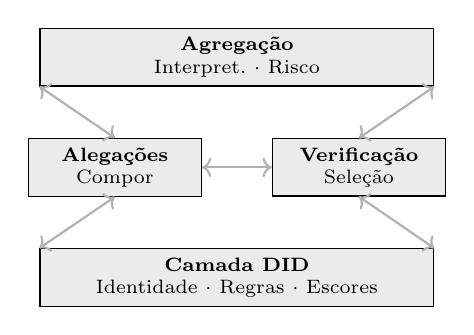
\begin{tikzpicture}[
    layer/.style={draw, minimum height=0.7cm, align=center, font=\scriptsize, fill=black!8},
    arr/.style={<->, thick, gray!60}
]
\node[layer, minimum width=5cm] (agg) at (0,2.8) {\textbf{Agregação}\\Interpret.\ $\cdot$ Risco};
\node[layer, minimum width=2.2cm] (claim) at (-1.55,1.4) {\textbf{Alegações}\\Compor};
\node[layer, minimum width=2.2cm] (verif) at (1.55,1.4) {\textbf{Verificação}\\Seleção};
\node[layer, minimum width=5cm] (did) at (0,0) {\textbf{Camada DID}\\Identidade $\cdot$ Regras $\cdot$ Escores};

\draw[arr] (agg.south west) -- (claim.north);
\draw[arr] (agg.south east) -- (verif.north);
\draw[arr] (claim.east) -- (verif.west);
\draw[arr] (claim.south) -- (did.north west);
\draw[arr] (verif.south) -- (did.north east);
\end{tikzpicture}
\caption{Arquitetura de quatro camadas da RSN.}
\label{fig:architecture}
\end{figure}

\subsection{Papéis dos Participantes}

Uma transação de verificação envolve até seis papéis distintos de DID (Fig.~\ref{fig:roles}): \textbf{Emissor} ($DID_I$, cria e submete a alegação), \textbf{Sujeito} ($DID_S$, o DID sobre o qual a alegação versa---pode coincidir com o Emissor), \textbf{Autoridade} ($DID_A$, endossa a alegação mediante taxa; pode também oferecer serviços de testemunho---\emph{opcional}), \textbf{Testemunha} ($DID_{W_{1..n}}$, monitor incógnito da honestidade do verificador por meio de códigos de desafio---\emph{opcional}), \textbf{Verificador} ($DID_V$, selecionado algoritmicamente para publicar a alegação) e a \textbf{RSN} (a rede onde as alegações verificadas são publicadas). Qualquer papel pode ser delegado a outro DID (Seção~7.4). Uma Autoridade comumente agrupa o endosso com serviços de testemunho, mas as duas funções são logicamente independentes.

\begin{figure}[ht]
\centering
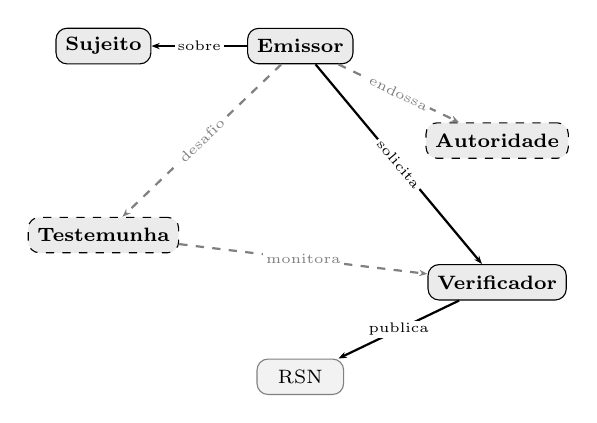
\begin{tikzpicture}[
    role/.style={draw, rounded corners, minimum width=1.1cm, minimum height=0.45cm, align=center, font=\scriptsize, fill=black!8},
    opt/.style={draw, rounded corners, minimum width=1.1cm, minimum height=0.45cm, align=center, font=\scriptsize, fill=black!8, dashed},
    arr/.style={-{Stealth[length=3pt]}, thick},
    oarr/.style={-{Stealth[length=3pt]}, thick, dashed, gray},
    lbl/.style={font=\tiny, fill=white, inner sep=1pt}
]
\node[role] (I) at (0,2.4) {\textbf{Emissor}};
\node[role] (S) at (-2.5,2.4) {\textbf{Sujeito}};
\node[opt] (A) at (2.5,1.2) {\textbf{Autoridade}};
\node[opt] (W) at (-2.5,0) {\textbf{Testemunha}};
\node[role] (V) at (2.5,-0.6) {\textbf{Verificador}};
\node[role, fill=black!5, draw=gray] (N) at (0,-1.8) {RSN};

\draw[arr] (I) -- node[lbl] {sobre} (S);
\draw[oarr] (I) -- node[lbl,sloped] {endossa} (A);
\draw[oarr] (I) -- node[lbl,sloped] {desafio} (W);
\draw[arr] (I) -- node[lbl,sloped] {solicita} (V);
\draw[oarr] (W) -- node[lbl] {monitora} (V);
\draw[arr] (V) -- node[lbl] {publica} (N);
\end{tikzpicture}
\caption{Papéis de DID em uma transação de verificação. Tracejado = opcional (Autoridade, Testemunha).}
\label{fig:roles}
\end{figure}

\subsection{Incorruptibilidade: Quatro Forças}

A incorruptibilidade da RSN não decorre de um único mecanismo, mas de quatro forças concorrentes. Nenhuma é suficiente por si só; apenas sua combinação torna economicamente irracional uma tentativa de corrupção.

\textbf{Alvo imprevisível.} O verificador de cada alegação é selecionado de forma não determinística por meio de hashing consistente (Seção~5.3). Um atacante não pode escolher previamente um verificador específico para suborno, porque a identidade do verificador é uma função do conteúdo da alegação e das iterações anteriores, não da escolha do emissor.

\textbf{Alavancagem reputacional---sobe devagar, cai depressa.} A reputação só pode ser ganha incrementalmente, por meio de comportamento consistente e sustentado. Ela pode, porém, ser perdida catastroficamente em um único endosso fraudulento (Seção~6.2). Essa assimetria significa que anos de reputação acumulada podem ser destruídos por um único endosso desonesto; a estratégia ótima continua sendo rejeitar alegações suspeitas.

\textbf{Promessa pública.} Todo Titular de DID declara publicamente sua política---um conjunto de regras legível por máquina que ele se compromete a seguir. A divergência entre a declaração e o comportamento real é detectável e precificada como uma infração reputacional mais grave do que a violação subjacente (Seção~7.3). A hipocrisia é, portanto, mais custosa do que a desonestidade direta.

\textbf{Assimetria de custo de ataque da malha.} O custo de censurar ou desestabilizar a rede cresce de forma não linear com o tamanho e a densidade da rede, ao passo que o custo de tolerá-la permanece constante. Para que a censura compensasse, um ator centralizado teria de aplicá-la sobre toda a rede---exigindo medidas desproporcionais a qualquer benefício concebível (Seção~10).

% ============================================================
% 4. DECENTRALIZED IDENTITY MODEL
% ============================================================
\section{Modelo de Identidade Descentralizada}

\subsection{DID com Propriedades Especiais}

A RSN estende a especificação W3C DID Core~\cite{did2022} com: \textbf{Regras Declaradas} (compromissos comportamentais legíveis por máquina), \textbf{Metadados de Reputação} (escore comportamental agregado) e \textbf{Roteamento de Rede} (gateway onion mutável, separado da posição estável no anel).

\subsection{Ciclo de Vida da Alegação}

Uma Alegação percorre seis estágios (Fig.~\ref{fig:lifecycle}): composição, endosso opcional por autoridade, seleção de verificador via hashing consistente, decisão de verificação (aceitar ou rejeitar com iteração), publicação e atualização de reputação para todas as partes.

\begin{figure}[ht]
\centering
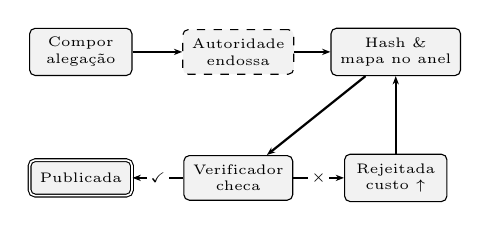
\begin{tikzpicture}[
    stp/.style={draw, rounded corners=2pt, minimum width=1.3cm, minimum height=0.45cm, align=center, font=\tiny, fill=black!5},
    arr/.style={-{Stealth[length=3pt]}, thick},
    lbl/.style={font=\tiny, fill=white, inner sep=1pt}
]
\node[stp] (comp) at (0,0) {Compor\\alegação};
\node[stp, dashed] (auth) at (2.0,0) {Autoridade\\endossa};
\node[stp] (hash) at (4.0,0) {Hash \&\\mapa no anel};
\node[stp] (ver) at (2.0,-1.6) {Verificador\\checa};
\node[stp, double] (pub) at (0,-1.6) {Publicada};
\node[stp] (rej) at (4.0,-1.6) {Rejeitada\\custo $\uparrow$};

\draw[arr] (comp) -- (auth);
\draw[arr] (auth) -- (hash);
\draw[arr] (hash) -- (ver);
\draw[arr] (ver) -- node[lbl] {\checkmark} (pub);
\draw[arr] (ver) -- node[lbl] {$\times$} (rej);
\draw[arr] (rej) -- ++(0,0.8) -| (hash);
\end{tikzpicture}
\caption{Ciclo de vida da alegação com laço de iteração.}
\label{fig:lifecycle}
\end{figure}

\subsection{Relação com o W3C DID Core}

O modelo de identidade da RSN é um superconjunto próprio da especificação W3C DID Core~\cite{did2022}. Todos os DIDs da RSN são DIDs W3C válidos. As extensões específicas da RSN são codificadas como propriedades do documento DID definidas em uma especificação de método DID dedicada, compatível com infraestruturas existentes como ION~\cite{buchner2021} e Ceramic~\cite{ceramic2023}.

% ============================================================
% 5. VERIFICATION AND PROPAGATION
% ============================================================
\section{Verificação e Propagação da Informação}

\subsection{Custo de Inserção de Informação}

O princípio econômico central da RSN é a assimetria entre ler e escrever. Ler dados de reputação aproxima-se de custo marginal zero para os participantes que fazem parte da rede DID e têm acesso proporcional à sua reputação---os recém-chegados devem conquistar gradualmente um acesso mais amplo (ver anti-parasitismo). Escrever---entendido como a materialização durável da reputação na rede, não como um ato técnico pontual---exige investimento cumulativo verificável em três dimensões: \textbf{tempo} (anos de vida despendidos em comportamento consistente, compromissos cumpridos e relacionamentos cultivados), \textbf{energia} (esforço investido em negociar com honestidade, no cuidado com as parcerias e na confiabilidade de longo prazo) e \textbf{dinheiro} (investimento no próprio nome---desenvolvimento profissional, qualidade do próprio trabalho, reparação dos danos causados). A reputação não pode ser comprada instantaneamente---ela é o resultado de uma acumulação ao longo da vida que o sistema apenas torna visível e transferível entre contextos. Os custos técnicos pontuais do protocolo (assinaturas criptográficas, taxas de verificador) são desprezíveis em comparação com esse investimento subjacente.

\subsection{Grafo Social e Profundidade de Contatos}

A RSN é fundamentalmente uma rede social: cada DID adiciona contatos (outros DIDs) que permitem a conexão. Esses contatos têm seus próprios contatos, e assim por diante. A busca algorítmica de verificadores opera dentro de uma profundidade configurável $h$ de contatos ligados (por exemplo, $h=3$: os contatos diretos de alguém, os contatos deles e os contatos dos contatos). Essa arquitetura não requer uma única blockchain global---ela favorece naturalmente o surgimento de comunidades/clusters com sobreposições em outras comunidades. Todo participante DID deve ter uma \textbf{política} publicada---um conjunto de regras legível por máquina que governa como as solicitações recebidas são avaliadas. As violações de política são registradas na rede como artefatos negativos.

\subsection{Seleção Algorítmica de Verificadores}

O protocolo de verificação emprega hashing consistente~\cite{karger1997} (Fig.~\ref{fig:verifier}). A verificação é um serviço pago: os verificadores operam mediante taxa, criando um mercado em que a concorrência impulsiona preço, velocidade e confiabilidade.

\textbf{Passo 1.} O documento da alegação é concatenado com o resultado do hash da iteração anterior (ou $\varnothing$ na primeira iteração) e submetido a hash:
\begin{equation}
\text{pos} = f_h(\text{claim} \| \text{prev\_hash})
\label{eq:hash}
\end{equation}

O algoritmo deve incluir o \emph{caminho completo} de todas as solicitações e respostas anteriores---não apenas um hash da iteração anterior. A resposta completa de cada verificador (aceitação, rejeição, preço cotado, motivo) é anexada ao documento em crescimento, verificável por meio de assinaturas criptográficas em cada etapa.

\textbf{Passo 2.} O hash é mapeado para $N$ posições no anel de hash consistente, distribuídas uniformemente (por exemplo, para $N=4$: $+0^{\circ}, +90^{\circ}, +180^{\circ}, +270^{\circ}$). A partir de cada posição, uma busca no sentido horário seleciona o DID mais próximo como candidato a verificador (Fig.~\ref{fig:multipoint}). $N$ é um parâmetro variável que pode depender do percentual de DIDs atualmente ativos, da hora do dia ou da capacidade de resposta histórica da rede.

\textbf{Passo 3.} O Verificador aceita (publica, apostando reputação) ou rejeita (retornando ao Passo~1 com o hash de rejeição). Quando um nó não responde apesar de declarar estar on-line, a solicitação seguinte deve incluir todas as respostas de todos os $N$ candidatos a verificador anteriores.

\textbf{Anti-parasitismo.} Os DIDs de destino podem estabelecer taxas ou restrições de acesso para consultas provenientes de DIDs novos com pouca reputação. Esse mecanismo gradual (não binário) obriga os recém-chegados a construir reputação por meio de atividade genuína antes de consumir livremente os dados alheios.

\begin{figure}[ht]
\centering
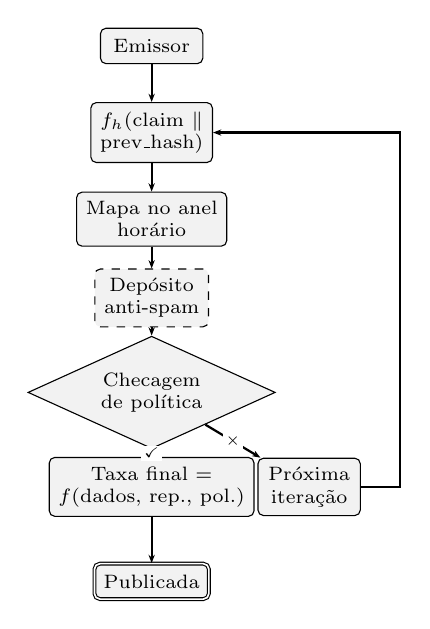
\begin{tikzpicture}[
    box/.style={draw, rounded corners=2pt, minimum width=1.3cm, minimum height=0.45cm, align=center, font=\scriptsize, fill=black!5},
    dec/.style={draw, diamond, aspect=2.2, minimum width=0.9cm, align=center, font=\scriptsize, fill=black!5},
    arr/.style={-{Stealth[length=3pt]}, thick},
    lbl/.style={font=\tiny, fill=white, inner sep=1pt}
]
\node[box] (iss) at (0,0) {Emissor};
\node[box] (hash) at (0,-1.1) {$f_h$(claim $\|$\\prev\_hash)};
\node[box] (ring) at (0,-2.2) {Mapa no anel\\horário};
\node[box, dashed] (spam) at (0,-3.2) {Depósito\\anti-spam};
\node[dec] (check) at (0,-4.4) {Checagem\\de política};
\node[box] (rej) at (2,-5.6) {Próxima\\iteração};
\node[box] (fee) at (0,-5.6) {Taxa final =\\$f$(dados, rep., pol.)};
\node[box, double] (pub) at (0,-6.8) {Publicada};

\draw[arr] (iss) -- (hash);
\draw[arr] (hash) -- (ring);
\draw[arr] (ring) -- (spam);
\draw[arr] (spam) -- (check);
\draw[arr] (check) -- node[lbl] {$\times$} (rej);
\draw[arr] (check) -- node[lbl] {\checkmark} (fee);
\draw[arr] (fee) -- (pub);
\draw[arr] (rej.east) -- ++(0.5,0) |- (hash.east);
\end{tikzpicture}
\caption{Protocolo de seleção de verificador. O depósito anti-spam é opcional e pode ser reembolsável. A taxa final é paga somente na aceitação.}
\label{fig:verifier}
\end{figure}

Cada rejeição anexa a resposta completa do verificador (incluindo motivos e condições) ao documento da alegação, expandindo seu conteúdo. A partir do documento expandido, um novo hash é computado de forma não determinística, mapeando para uma posição diferente no anel e selecionando um verificador diferente. A documentação do caminho completo é obrigatória---o emissor não pode prever nem influenciar o próximo verificador. Se um verificador ignora uma solicitação apesar de uma política declarada compatível, as testemunhas (se presentes) registram isso, e o emissor pode anexar a evidência das testemunhas na publicação final.

\begin{figure}[ht]
\centering
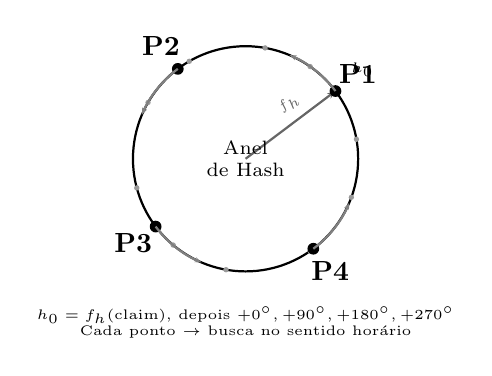
\begin{tikzpicture}[scale=0.65]
% Ring
\draw[thick] (0,0) circle (2.2cm);
% DID nodes on ring
\foreach \a in {10,55,80,120,150,195,230,260,305,340} {
  \fill[black!40] (\a:2.2) circle (1.5pt);
}
% Hash offset arrow pointing to initial position
\draw[-{Stealth[length=3pt]}, thick, black!60] (0,0) -- node[font=\tiny,above,sloped,pos=0.6] {$f_h$} (37:2.2);
\fill[black] (37:2.2) circle (2pt);
\node[font=\tiny,anchor=south west] at (37:2.35) {$h_0$};
% N=4 points offset from h0 by +0, +90, +180, +270
\foreach \offset/\l in {0/P1,90/P2,180/P3,270/P4} {
  \pgfmathsetmacro{\ang}{37+\offset}
  \node[fill=black, circle, inner sep=1.5pt] (p\offset) at (\ang:2.2) {};
  \node[font=\tiny,font=\bfseries] at (\ang:2.75) {\l};
  % clockwise search arc
  \draw[-{Stealth[length=2.5pt]}, thick, gray] (\ang:2.2) arc (\ang:\ang+30:2.2);
}
\node[font=\scriptsize, align=center] at (0,0) {Anel\\de Hash};
\node[font=\tiny, align=center] at (0,-3.2) {$h_0 = f_h(\text{claim})$, depois $+0^{\circ},+90^{\circ},+180^{\circ},+270^{\circ}$\\Cada ponto $\rightarrow$ busca no sentido horário};
\end{tikzpicture}
\caption{Seleção multiponto ($N{=}4$). O hash $h_0$ define o deslocamento; 4 pontos distribuídos uniformemente a partir de $h_0$.}
\label{fig:multipoint}
\end{figure}

\subsection{Protocolo de Testemunho}

O papel de \textbf{Testemunha} fornece responsabilização incógnita para a honestidade do verificador por meio de um protocolo criptográfico de código de desafio:

\textbf{Passo W1.} O solicitante assina a solicitação de verificação e a envia a $N_w$ testemunhas---contatos da rede social do solicitante ou provedores especializados de serviço de testemunho que operam mediante taxa.

\textbf{Passo W2.} Cada testemunha $w_i$ assina toda a solicitação assinada, retém a assinatura original $\sigma_i$ e computa um código de desafio $c_i = h(\sigma_i)$. O código de desafio é anexado à solicitação.

\textbf{Passo W3.} A solicitação, agora carregando $N_w$ códigos de desafio, é enviada ao verificador. O verificador observa os códigos, mas \emph{não consegue determinar} quem são as testemunhas nem se os códigos correspondem a assinaturas reais.

\textbf{Passo W4 (verificador honesto).} Se o verificador responde de acordo com sua política declarada, os códigos de desafio permanecem opacos. As testemunhas nunca são reveladas. Nenhum dado adicional é publicado.

\textbf{Passo W5 (violação de política).} Se o verificador viola sua política (ignora a solicitação, responde de forma inconsistente), o solicitante detém as assinaturas originais das testemunhas $\sigma_i$. Estas podem ser publicadas como dados complementares: qualquer um pode verificar $c_i = h(\sigma_i)$, provando que a testemunha estava presente. O solicitante pode publicar de forma independente---o verificador já assinou os códigos de desafio em sua resposta.

\textbf{A propriedade do blefe.} O solicitante pode substituir alguns ou todos os códigos de desafio por valores aleatórios. O verificador não consegue distinguir códigos genuínos (respaldados por autoridades de alta reputação) de ruído. Essa \emph{incerteza} é o mecanismo de execução: toda solicitação carrega o risco de que uma autoridade respeitada esteja observando de forma incógnita. O custo de manter essa pressão é quase nulo (gerar números aleatórios), enquanto o custo potencial da desonestidade para o verificador é catastrófico. O comportamento honesto é incentivado mesmo na ausência de testemunhas reais.

\textbf{Autoridade como testemunha.} Uma Autoridade que endossa uma alegação pode agrupar serviços de testemunho: ``Endosso sua alegação e sirvo como testemunha incógnita durante a verificação.'' Esse é um modelo de negócio natural---a Autoridade já dispõe do contexto. No entanto, os dois papéis são logicamente independentes.

\subsection{Princípio do Radicalismo Custoso}

Três canais de custo se acumulam simultaneamente (Fig.~\ref{fig:radicalism}):

\textbf{Canal 1: Custo de Iteração.} Cada rejeição força uma nova iteração que consome tempo e recursos. Crescimento linear.

\textbf{Canal 2: Inchaço do Documento.} Cada iteração adiciona a resposta completa do verificador ao documento da alegação. O crescimento é linear, mas com um deslocamento de base: a carga inicial (conteúdo da alegação, endosso de autoridade, assinaturas criptográficas) já tem tamanho não trivial $B_0$. Tamanho total após $k$ iterações: $S(k) = B_0 + k \cdot \Delta$, onde $\Delta$ é o tamanho médio da resposta.

\textbf{Canal 3: Prêmio de Risco do Verificador.} O risco é subjetivo. O verificador avalia se as políticas declaradas do DID solicitante conflitam com os interesses comerciais, sociais ou políticos do próprio verificador. O prêmio pode escalar exponencialmente com a distância percebida em relação ao ``ideal'' do verificador: $P(d) = \alpha \cdot e^{\beta d}$, onde $d$ é a métrica de distância subjetiva do verificador. Além de um limite pessoal intransponível, o verificador pode recusar por completo.

\begin{figure}[ht]
\centering
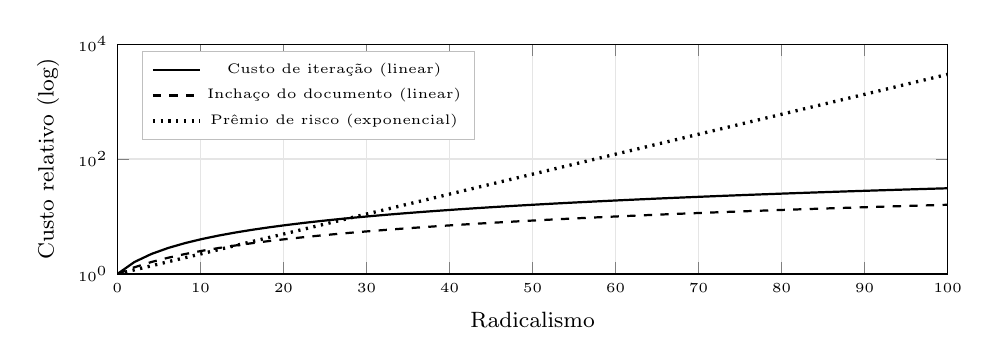
\begin{tikzpicture}
\begin{axis}[
    width=\columnwidth,
    height=4.5cm,
    xlabel={\footnotesize Radicalismo},
    ylabel={\footnotesize Custo relativo (log)},
    ymode=log,
    xmin=0, xmax=100,
    ymin=1, ymax=10000,
    grid=major,
    grid style={gray!20},
    legend style={at={(0.03,0.97)},anchor=north west,font=\tiny,draw=gray!50},
    tick label style={font=\tiny},
    label style={font=\footnotesize},
]
\addplot[black, thick, domain=0:100, samples=50] {1 + 0.3*x};
\addlegendentry{Custo de iteração (linear)}
\addplot[black, thick, dashed, domain=0:100, samples=50] {1 + 0.15*x};
\addlegendentry{Inchaço do documento (linear)}
\addplot[black, thick, dotted, line width=1.2pt, domain=0:100, samples=100] {exp(0.08*x)};
\addlegendentry{Prêmio de risco (exponencial)}
\end{axis}
\end{tikzpicture}
\caption{Escalada de custo ao longo de três canais. O prêmio de risco domina em alto radicalismo.}
\label{fig:radicalism}
\end{figure}

Crucialmente, isso não é censura. Nenhuma alegação é proibida. O sistema precifica o risco (Tabela~\ref{tab:costs}).

\begin{table}[ht]
\centering
\caption{Comparação de custos entre tipos de alegação.}
\label{tab:costs}
\footnotesize
\begin{tabular}{@{}lcccc@{}}
\toprule
\textbf{Tipo} & \textbf{Iter.} & \textbf{Doc} & \textbf{Taxa} & \textbf{Total} \\
\midrule
Crível & $k_{\min}$ & $B_0$ & $P_{\min}$ & Baixo \\
Controversa & $k_{\text{med}}$ & $B_0{+}k\Delta$ & $\alpha e^{\beta d}$ & Moderado \\
Radical & $k_{\max}$ & $\gg B_0$ & $\gg P_{\min}$ & Muito alto \\
Fraudulenta & $\to\infty$ & --- & --- & Impublicável \\
\bottomrule
\end{tabular}
\end{table}

% ============================================================
% 6. REPUTATION AND RISK
% ============================================================
\section{Reputação e Avaliação de Risco}

\subsection{Modelo de Acumulação de Reputação}

A reputação exibe três propriedades: \textbf{acumulação lenta} (crescimento incremental por meio de comportamento consistente), \textbf{destruição rápida} (uma única fraude pode reduzir o escore catastroficamente) e \textbf{avaliação individual} (cada parte consumidora pode aplicar sua própria função de agregação).

\subsection{Autoridades Reputáveis}

Uma Autoridade Reputável revisa alegações e, se satisfeita, coassina-as---apostando sua própria reputação (Fig.~\ref{fig:authority}). A assimetria é intencional: ganhar reputação é lento (incremento $+\delta$ por endosso honesto), enquanto perdê-la é catastrófico ($-\Delta \gg \delta$ por endosso falso; a título ilustrativo, por exemplo, $+2\%$ contra $-70\%$). A estratégia ótima é sempre rejeitar alegações suspeitas. Os valores específicos de $\delta$ e $\Delta$ são parâmetros do sistema.

\begin{figure}[ht]
\centering
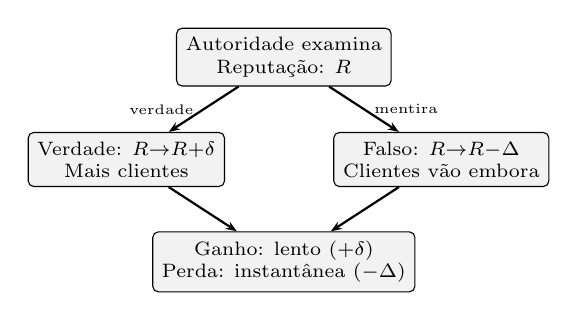
\begin{tikzpicture}[
    box/.style={draw, rounded corners=2pt, minimum width=2cm, minimum height=0.6cm, align=center, font=\scriptsize, fill=black!5},
    arr/.style={-{Stealth[length=4pt]}, thick}
]
\node[box] (exam) at (0,0) {Autoridade examina\\Reputação: $R$};
\node[box] (true) at (-2,-1.3) {Verdade: $R{\to}R{+}\delta$\\Mais clientes};
\node[box] (false) at (2,-1.3) {Falso: $R{\to}R{-}\Delta$\\Clientes vão embora};
\node[box] (insight) at (0,-2.6) {Ganho: lento ($+\delta$)\\Perda: instantânea ($-\Delta$)};

\draw[arr] (exam) -- node[left,font=\tiny] {verdade} (true);
\draw[arr] (exam) -- node[right,font=\tiny] {mentira} (false);
\draw[arr] (true) -- (insight);
\draw[arr] (false) -- (insight);
\end{tikzpicture}
\caption{Autoridade Reputável---incentivos assimétricos.}
\label{fig:authority}
\end{figure}

\subsection{Reputação Multidimensional}

A reputação não é um escalar, mas um vetor ao longo de múltiplas dimensões: confiabilidade financeira, integridade pessoal, competência profissional, engajamento cívico e outras (Fig.~\ref{fig:reputation-radar}). Diferentes provedores de avaliação projetam esse vetor de maneira distinta conforme o contexto---um credor prioriza a confiabilidade financeira, um empregador a competência profissional, um vizinho o comportamento cívico. Não existe um único escore de reputação ``correto''; apenas perspectivas.

\begin{figure}[ht]
\centering
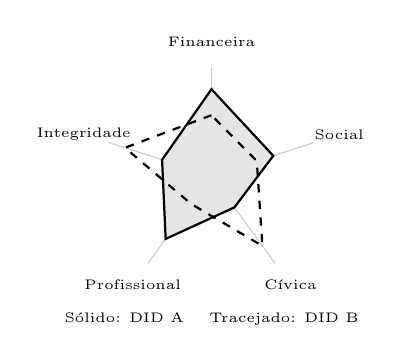
\begin{tikzpicture}[scale=0.55]
\foreach \a/\l in {90/Financeira,162/Integridade,234/Profissional,306/Cívica,18/Social} {
  \draw[gray!40] (0,0) -- (\a:2.5);
  \node[font=\tiny, align=center] at (\a:3.1) {\l};
  \foreach \r in {0.8,1.6,2.4} {
    \fill[black!15] (\a:\r) circle (0.5pt);
  }
}
\draw[thick, fill=black!10] (90:2.0) -- (162:1.2) -- (234:1.8) -- (306:0.9) -- (18:1.5) -- cycle;
\draw[thick, dashed] (90:1.4) -- (162:2.1) -- (234:0.8) -- (306:2.0) -- (18:1.1) -- cycle;
\node[font=\tiny] at (0,-3.3) {Sólido: DID A \quad Tracejado: DID B};
\end{tikzpicture}
\caption{Vetores de reputação multidimensionais. Diferentes DIDs exibem perfis diferentes ao longo das dimensões.}
\label{fig:reputation-radar}
\end{figure}

\subsection{Avaliação de Risco Democratizada}

A RSN democratiza a avaliação sistemática de risco---uma capacidade hoje concentrada nas instituições financeiras, mas aplicável muito além do setor bancário. Conglomerados industriais avaliando a confiabilidade de fornecedores, seguradoras precificando o risco comportamental, due diligence para fusões e aquisições, estimativa de vida útil de equipamentos na indústria---em qualquer lugar em que o risco da contraparte precise ser avaliado, a RSN oferece uma alternativa descentralizada e orientada pelo mercado. Um mercado de serviços de interpretação traduz dados brutos de reputação multidimensional em resumos acionáveis, tornando a avaliação da contraparte acessível a qualquer participante a custo marginal.

% ============================================================
% 7. CONSENSUS AND DISPUTE RESOLUTION
% ============================================================
\section{Consenso e Resolução de Disputas}

\subsection{Modelo de Justiça Descentralizada}

A RSN reformula a justiça como um problema de negociação bilateral. A ameaça de um dano reputacional permanente e verificável é um dissuasor mais eficaz do que ações judiciais que a parte lesada não pode custear.

\subsection{Consenso Emergente}

Cada participante mantém um limiar pessoal de satisfação. O consenso agregado da rede emerge como a média estatística de milhares de negociações bilaterais (Fig.~\ref{fig:consensus}). Uma resposta muito acima do consenso (bárbara) é cara de publicar. Uma resposta próxima ao consenso (proporcional) é barata. O consenso não é uma regra---é um sinal de preço.

\begin{figure}[ht]
\centering
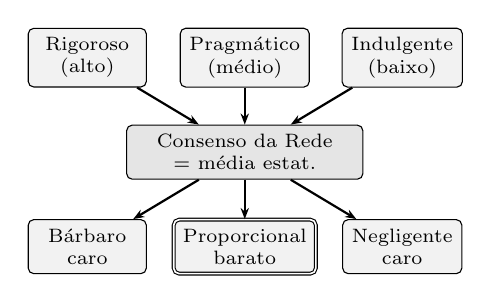
\begin{tikzpicture}[
    person/.style={draw, rounded corners=2pt, minimum width=1.5cm, minimum height=0.5cm, align=center, font=\scriptsize, fill=black!5},
    arr/.style={-{Stealth[length=4pt]}, thick}
]
\node[person] (a) at (-2,0) {Rigoroso\\(alto)};
\node[person] (b) at (0,0) {Pragmático\\(médio)};
\node[person] (c) at (2,0) {Indulgente\\(baixo)};
\node[person, fill=black!10, minimum width=3cm] (cons) at (0,-1.2) {Consenso da Rede\\= média estat.};
\node[person] (exp) at (-2,-2.4) {Bárbaro\\caro};
\node[person, double] (prop) at (0,-2.4) {Proporcional\\barato};
\node[person] (neg) at (2,-2.4) {Negligente\\caro};

\draw[arr] (a) -- (cons);
\draw[arr] (b) -- (cons);
\draw[arr] (c) -- (cons);
\draw[arr] (cons) -- (exp);
\draw[arr] (cons) -- (prop);
\draw[arr] (cons) -- (neg);
\end{tikzpicture}
\caption{Consenso emergente a partir dos limiares individuais de satisfação.}
\label{fig:consensus}
\end{figure}

\subsection{Calibração da Punição}

Cada Titular de DID declara publicamente respostas a categorias específicas de má conduta. Declarações desproporcionalmente severas ou brandas atraem sinais reputacionais negativos. Declarações proporcionais são aceitas sem atrito---um sistema de punição autocalibrável.

As declarações de consenso estão elas próprias sujeitas à detecção de hipocrisia: comprometer-se declarativamente com uma posição de consenso enquanto se comporta de forma inconsistente constitui uma infração reputacional mais grave do que o próprio desvio subjacente, pois demonstra engano intencional.

\subsection{Delegação}

Todas as atividades dentro de um DID---com uma exceção---podem ser delegadas a outro DID. \textbf{O papel de Sujeito---o DID cujo comportamento é objeto da alegação---não pode ser delegado; ele está intransferivelmente vinculado ao titular da identidade a quem a alegação se refere.} Os demais papéis ativos---Emissor, Autoridade, Testemunha, Verificador---podem ser transferidos a um DID delegado designado, seja para verificação, submissão de alegação, participação no consenso ou resolução de disputas. A delegação é revogável a qualquer momento. Isso possibilita a especialização (por exemplo, serviços profissionais de verificação) enquanto o Titular mantém o controle e a responsabilidade em última instância. A delegação aplica-se a todo o sistema e é essencial para a escalabilidade.

\subsection{Da Moralidade Individual ao Contrato Social Emergente}

A política declarada de cada DID representa uma formalização da moralidade individual: o que o Titular considera aceitável, como responde a comportamentos específicos, o que exige das contrapartes. Essas políticas não são impostas por um projetista do sistema---são escolhidas por cada participante e expressas em forma legível por máquina.

Essa formalização possibilita uma emergência em três estágios. Primeiro, a moralidade individual é codificada como \textbf{política}---um conjunto de regras declaradas, limiares e funções de resposta que o DID se compromete a seguir. Segundo, o agregado de todas as políticas ao longo da rede produz \textbf{ética emergente}---normas estatisticamente observáveis que nenhum participante isolado projetou, mas que surgem da interação de milhares de posições morais individuais~\cite{durkheim1893}. Terceiro, essa ética emergente, expressa como normas comportamentais compartilhadas e executada por meio de sinais de preço bilaterais, constitui um \textbf{contrato social mensurável}---não um construto teórico que ninguém assinou~\cite{rawls1971}, mas um conjunto de regras empiricamente observável e respaldado por comportamento efetivo.

Esse processo espelha achados da teoria das fundações morais~\cite{haidt2012}: a moralidade humana é intuitiva, pluralista e culturalmente variável. A RSN não requer consenso moral como entrada; ela produz consenso comportamental como saída. O contrato social resultante não é estático---ele evolui à medida que os participantes entram, saem e ajustam suas políticas em resposta à retroalimentação da rede. Diferentemente da teoria clássica do contrato social, esse contrato é revogável, observável e executável sem um soberano.

% ============================================================
% 8. ECONOMIC MODEL
% ============================================================
\section{Modelo Econômico}

As seções anteriores descreveram uma ferramenta---os mecanismos de verificação, a estrutura de custo e o consenso emergente da RSN. Esta seção descreve uma metodologia para aplicar essa ferramenta à transição fiscal e de governança. A ferramenta é de propósito geral; a metodologia a seguir é uma aplicação possível.

\subsection{Estrutura de Incentivos}

A reputação como capital cria incentivos diretos ao comportamento honesto. Em operação normal, os participantes constroem reputação naturalmente por meio de transações cotidianas e compromissos cumpridos. O principal dispêndio ocorre com alegações \emph{negativas}---o registro de danos causados por outros. Essa assimetria incentiva o comportamento útil e confiável: ser honesto não custa nada extra, enquanto ser danoso cria um rastro documentado que outros pagarão para preservar. A hipocrisia---declarar regras sem segui-las---é o modo de falha mais caro, pois demonstra engano intencional.

\subsection{Sistema Fiscal Paralelo}

Três componentes permitem a pressão competitiva: (1)~\textbf{Imposto Simples}---uma alíquota proporcional única, sem exceções, inicialmente marginalmente abaixo da alíquota efetiva vigente; (2)~\textbf{Registro Eletrônico de Gastos (REG)}---invertendo o modelo tcheco EET para que os cidadãos fiscalizem os gastos do Estado; (3)~\textbf{Destinação Tributária Dirigida pelo Cidadão}---começando com alguns pontos percentuais no primeiro ano e alcançando, após uma década, algo entre os dois dígitos baixos e uma migração completa para um sistema dirigido pelo cidadão, conforme o ritmo de adoção. O tempo efetivo depende da velocidade com que surgem alternativas de livre mercado aos serviços estatais e da disposição do Estado em cooperar com a transição; a função do tempo não precisa ser linear, e não há razão para estabelecer um limite superior para onde a adoção pode, em última instância, chegar.

% ============================================================
% 9. MIGRATION PATH
% ============================================================
\section{Caminho de Migração}

A migração procede por três fases (Fig.~\ref{fig:migration}): \textbf{Fase~1: Sobreposição} (a RSN como camada informacional, o Estado é o provedor exclusivo), \textbf{Fase~2: Concorrência} (a RSN oferece alternativas funcionais, uso de sistema duplo) e \textbf{Fase~3: Transição} (a RSN supera os equivalentes estatais, migração voluntária). A transição é reversível em cada etapa.

\begin{figure}[ht]
\centering
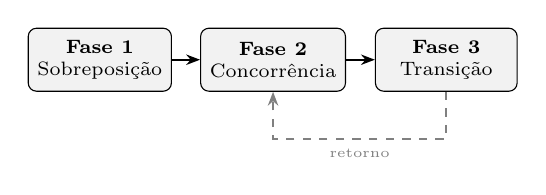
\begin{tikzpicture}[
    phase/.style={draw, rounded corners=3pt, minimum width=1.8cm, minimum height=0.8cm, align=center, font=\scriptsize, fill=black!5},
    arr/.style={-{Stealth[length=5pt]}, thick}
]
\node[phase] (p1) at (0,0) {\textbf{Fase 1}\\Sobreposição};
\node[phase] (p2) at (2.2,0) {\textbf{Fase 2}\\Concorrência};
\node[phase] (p3) at (4.4,0) {\textbf{Fase 3}\\Transição};

\draw[arr] (p1) -- (p2);
\draw[arr] (p2) -- (p3);
\draw[arr, dashed, gray] (p3.south) -- ++(0,-0.6) -| node[below,font=\tiny,pos=0.25] {retorno} (p2.south);
\end{tikzpicture}
\caption{Migração em três fases---reversível em cada etapa.}
\label{fig:migration}
\end{figure}

O principal mecanismo de pressão é fiscal: quando os contribuintes condicionais atingem uma ``minoria economicamente significativa $X$''---um grupo grande o bastante para que a repressão contra ele cause dano econômico não trivial e a desobediência civil se torne uma ameaça crível---o Estado entra em negociação. Para fins de ilustração, usamos $X \approx 15\%$ do PIB, mas o limiar efetivo depende da economia específica.

% ============================================================
% 10. SECURITY ANALYSIS
% ============================================================
\section{Análise de Segurança}

Consideramos cinco categorias de adversários: maus atores individuais, grupos organizados, adversários corporativos, adversários de nível estatal e adversários de nível de protocolo.

\textbf{Resistência a Sybil}~\cite{douceur2002}. Construir reputação exige interação sustentada e verificável. O custo de um ataque Sybil bem-sucedido escala linearmente com o número de identidades falsas e quadraticamente com o nível de reputação almejado. Operar múltiplos DIDs em paralelo é possível, mas caro por projeto---cada identidade deve acumular reputação de forma independente por meio de atividade genuína. Em sociedades livres, esse custo dissuade o abuso casual; em ditaduras, os DIDs paralelos tornam-se uma ferramenta de sobrevivência que possibilita resistência compartimentada, coordenação clandestina e navegação mais segura no mercado negro.

\textbf{Defesa contra conluio.} Padrões de endosso mútuo entre grupos fechados são detectáveis por meio da análise do grafo social. As funções de agregação de reputação descontam alegações provenientes de fontes densamente aglomeradas.

\textbf{Adversário de nível estatal.} O roteamento onion, a ausência de infraestrutura centralizada e a distribuição do papel de Verificador por toda a base de participantes garantem que a supressão exija medidas desproporcionais a qualquer benefício.

\textbf{Privacidade vs.\ responsabilização.} O pseudonimato---um meio-termo entre o anonimato e a divulgação da identidade---permite que os DIDs acumulem reputação significativa sem revelar a identidade real do Titular no mundo.

% ============================================================
% 11. PRIVACY
% ============================================================
\section{Considerações sobre Privacidade}

O modelo de privacidade da RSN é construído sobre o pseudonimato. O Titular controla a divulgação da identidade: mínima (pseudônimo puro), seletiva (credenciais específicas vinculadas) ou plena (identidade legal associada). As alegações publicadas são permanentes---o sistema suporta correção contextual, mas não apagamento. Um Titular pode abandonar um DID comprometido e recomeçar, abrindo mão da reputação acumulada.

% ============================================================
% 12. RELATED WORK
% ============================================================
\section{Trabalhos Relacionados}

A especificação W3C DID Core~\cite{did2022} e a Ceramic Network~\cite{ceramic2023} fornecem a base de identidade. O EigenTrust~\cite{kamvar2003} demonstrou a agregação distribuída de reputação sem autoridade central. Os SBTs~\cite{weyl2022} introduziram tokens sociais intransferíveis. A RSN difere na sua ênfase no custo econômico como filtro de qualidade e no seu mecanismo de precificação do radicalismo.

As DAOs~\cite{buterin2014} e o voto quadrático~\cite{buterin2019} demonstraram a viabilidade da governança descentralizada. A RSN deriva o consenso de negociações bilaterais de preço, em vez de votação.

A proposta baseia-se na teoria anarcocapitalista~\cite{rothbard1973,hoppe2001} para a provisão privada de serviços, mas dela se afasta em dois aspectos críticos: projeta para o rancor e os impulsos retributivos em vez de supor racionalidade, e propõe uma transição gradual em vez de revolução. O conceito de contratos sociais emergentes tem antecedentes na teoria da ordem espontânea de Hayek~\cite{hayek1973}.

\textbf{Anarco-agorismo.} A RSN compartilha um significativo terreno comum com a contraeconomia agorista~\cite{konkin2006}---particularmente a ênfase na construção de instituições paralelas e na troca voluntária. No entanto, o agorismo tende a supor o interesse próprio racional como mecanismo de coordenação suficiente e frequentemente carece de um caminho concreto de migração a partir das estruturas estatais existentes. A RSN incorpora explicitamente tendências comportamentais não racionais e fornece um mecanismo de pressão fiscal para uma transição gradual.

\textbf{Meritocracia.} A RSN pode representar uma primeira descrição funcional de como a meritocracia~\cite{young1958} pode emergir como uma propriedade sistêmica, e não como um slogan. Os sistemas meritocráticos tradicionais falham porque exigem uma autoridade central para definir e fazer valer o ``mérito''. Na RSN, o mérito emerge de avaliações bilaterais: aqueles que entregam valor acumulam reputação; nenhum comitê decide quem tem mérito.

\textbf{Propriedade como privilégio.} A RSN afasta-se fundamentalmente dos tratamentos anarcocapitalistas e da escola austríaca sobre os direitos de propriedade como naturais e absolutos. No arcabouço da RSN, a propriedade é um \emph{privilégio}---um reconhecimento social que pode, em casos extremos, ser retirado pela comunidade quando um participante viola fundamentalmente normas compartilhadas (traição, recusa em defender a comunidade em crise existencial, exploração sistemática). Isso não é expropriação estatal, mas a retirada do reconhecimento social pela rede de relações bilaterais.

% ============================================================
% 13. LIMITATIONS
% ============================================================
\section{Discussão e Limitações}

\textbf{Partida a frio.} O valor da RSN depende de efeitos de rede; os primeiros a adotá-la enfrentam valor limitado até que a participação atinja um limiar. Contudo, mesmo desde os estágios iniciais, a rede DID serve como uma útil fonte suplementar de informação. Espera-se que a avaliação inicial de reputação e a aferição de autoridade se desenvolvam gradualmente, com sofisticação crescente.

\textbf{Anti-parasitismo e controle de acesso.} Os DIDs de destino podem impor taxas graduadas e restrições de acesso a consultas provenientes de DIDs de baixa reputação. Isso não é binário, mas uma escala contínua: quanto menos reputação um DID consultante tem, menos informação recebe, mais tempo espera e mais paga. Esse mecanismo incentiva a participação genuína em vez do consumo passivo.

\textbf{Desigualdade de acesso.} O custo de publicar alegações pode filtrar queixas legítimas de participantes economicamente desfavorecidos. Mitigação: todo participante serve simultaneamente como verificador em potencial (ou delega esse papel) e aufere taxas de verificação. Ao longo de um horizonte de tempo suficiente, um participante não radical deveria aproximar-se da neutralidade financeira---a renda de verificação compensando aproximadamente os custos de publicação. Trata-se de uma expectativa estatística, não de uma garantia.

\textbf{Desigualdade de reputação.} Os primeiros a adotar acumulam vantagens que podem criar barreiras para os retardatários. No entanto, a avaliação de reputação é realizada por provedores terceiros, que podem optar por mitigar a vantagem do pioneiro por meio de seus algoritmos de agregação. Ser o primeiro com boa reputação é uma vantagem econômica comparativa legítima---e isso é intencional.

\textbf{Questões em aberto.} Funções de custo ótimas, padrões de agregação, governança do protocolo e a interação com dados de reputação sintética gerados por IA permanecem áreas para trabalho futuro.

Este artigo não afirma que a RSN produzirá resultados ótimos em todas as circunstâncias. Ele afirma que a RSN representa uma alternativa \emph{viável}---tecnicamente implementável, economicamente autossustentável e socialmente compatível com as tendências comportamentais humanas tais como realmente são.

% ============================================================
% 14. CONCLUSION
% ============================================================
\section{Conclusão}

Este artigo apresentou a Rede Social de Reputação, um protocolo descentralizado que possibilita a troca pseudônima e verificável de reputação. O Princípio do Radicalismo Custoso garante que alegações fraudulentas sejam precificadas para fora do sistema, sem censura. O caminho de migração proposto viabiliza uma transição gradual e reversível a partir das instituições existentes. O projeto incorpora a natureza humana tal como ela é---incluindo a mesquinhez, o rancor e o desejo de satisfação retributiva---em vez de exigir uma transformação ideológica. O resultado não é a utopia, mas um sistema em que a justiça é acessível, a reputação é conquistada e o custo da má conduta é arcado pela parte que o causou.

% ============================================================
% REFERENCES
% ============================================================
\bibliography{references}

\end{document}
